\chapter{Sensor PCB assembly}

\section{Sensor PCB version 1.2}

\section{Order of assembly}
Fit components in this order:
\begin{itemize}
\item IC1 (MAXMCP3424).
\item IC2 (MAX619).
\item Turned pin sockets for the FLC100 sensor. Accurate alignment is
  importa so use a peice of solderless breadboard to hold the male pin
  headers, which hold the female headers vertical and correctly
  spaced. Place the circuit board upside down and solder to the female
  header. Only remove the male pin headers when the female header is
  fully soldered.
\item R1, R2, R3 (\kohm{10}).
\item R4 (\kohm{100}).
\item R5 (\kohm{4.7}).
\item C1, C2, C5, C9 (\nF{100}).
\item C9 (\nF{10}).  
\item C6, C7 (\nF{220}).
\item C3, C4 (\uF{4.7}).
\item D1 (BAT85).
\item SENS2 (LM61).
\item JP5 and JP7 (fit as $2\times3$ male header).
\item X1 (RJ45 vertical jack).
\item \warningbox{Q1 (2N7000). This item is very sensitive to damage
    by electrostatic discharge!}
\end{itemize}

\begin{landscape}
  % \thispagestyle{empty}
  \begin{figure}[p]
    \centering
    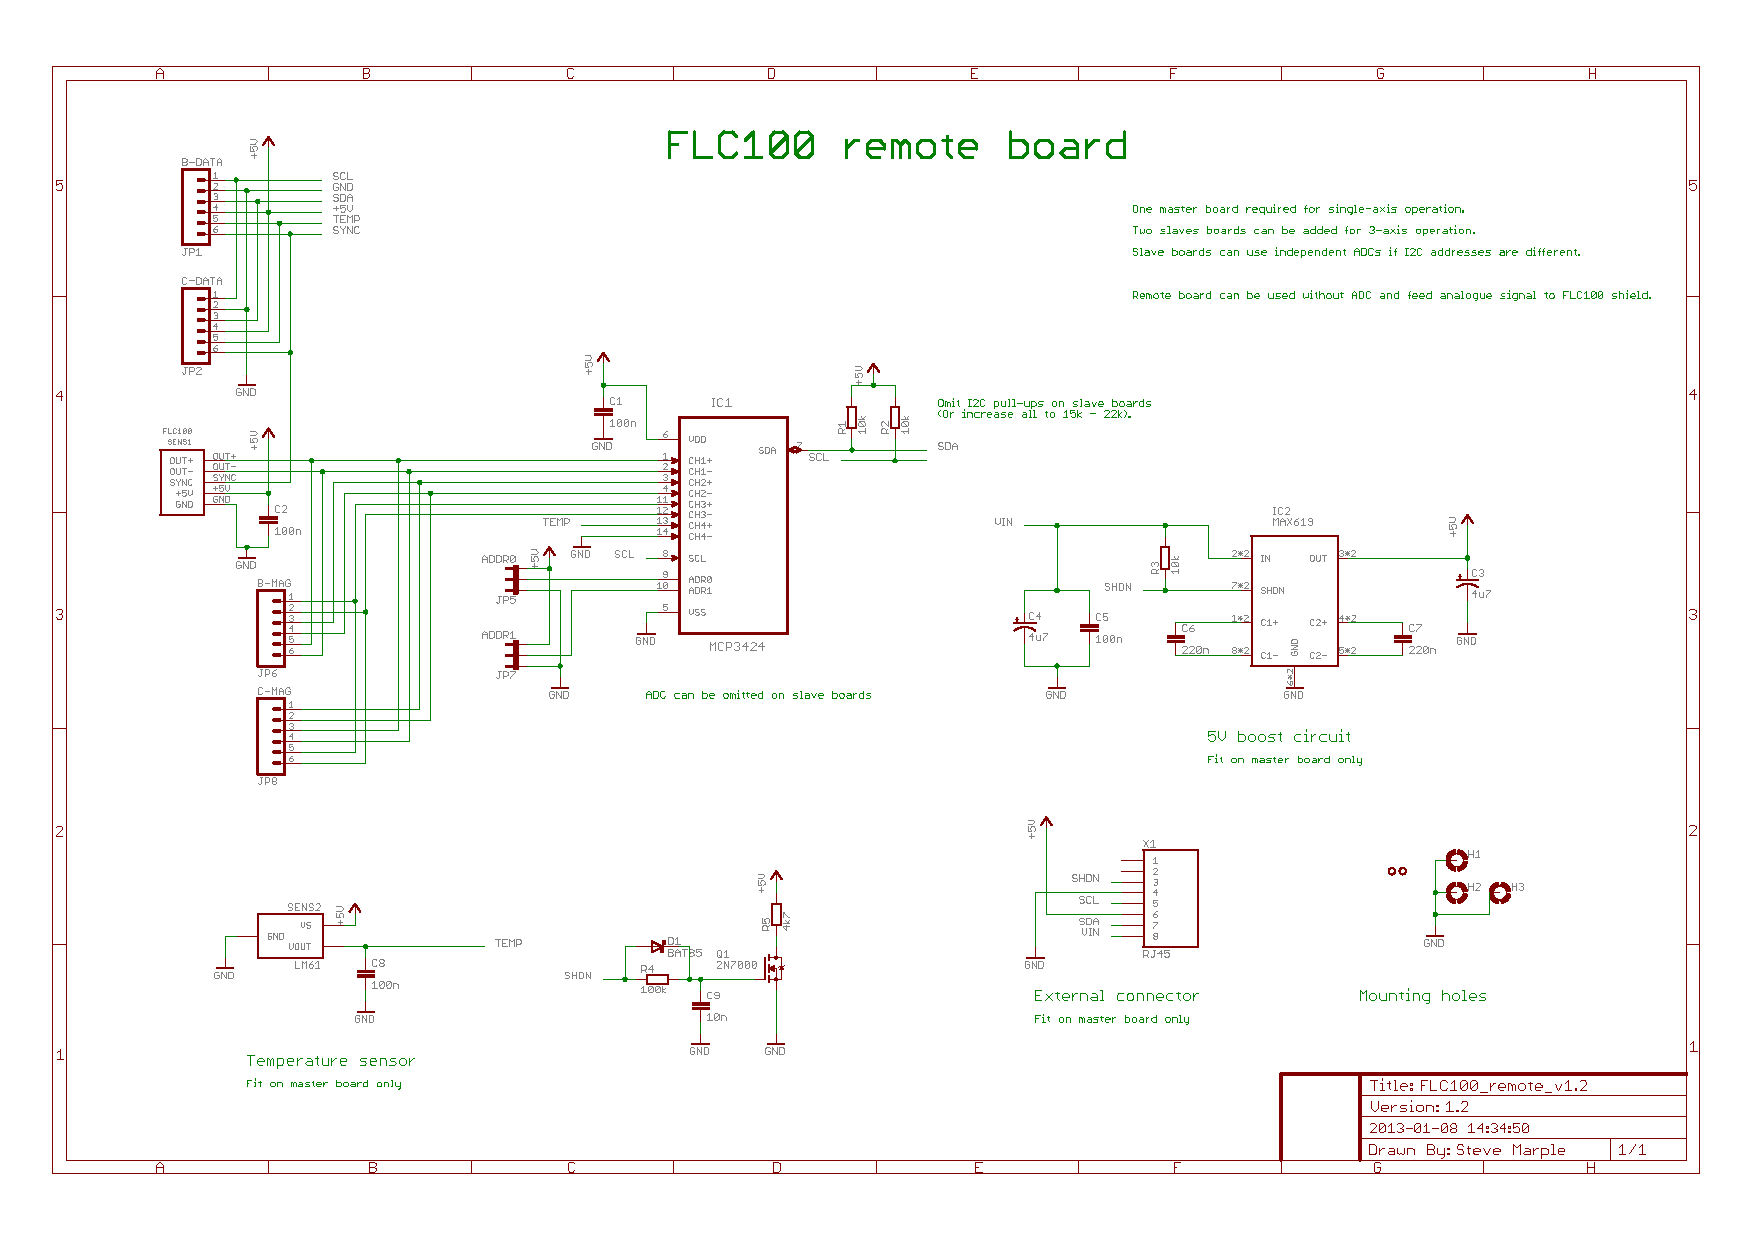
\includegraphics[keepaspectratio,width=28cm,height=16cm]{%
      {../../hardware/FLC100_shield/remote_v1.2/FLC100_remote_v1.2_sch}.pdf}
    \caption{Sensor PCB version 1.2 circuit diagram.}
    \label{fig:sensor-v1.2-pcb-cct-diag}
  \end{figure}
\end{landscape}
